
\chapter{TCN and Transformer}

\section{Temporal Convolutional Networks (TCN)}
A sequence model is a model that takes in input a sequence of items (words, letters, time series, audio signals, etc.) and produces an output sequence. Traditional models for sequence modeling include Recurrent Neural Networks (RNNs) and Long Short-Term Memory networks (LSTMs). But recent result indicate that other neural network architectures can outperform this tradutional models.
Typiccaly the name of a single item that give the sequence is a \textbf{token}.

\subsection{Use of Convolutions for Sequence Modeling}
The standard Convolutional Neural Network was first introduced in the LeNet-5 architecture.
Conv2D is generally used on image data. It is called 2-dimensional CNN because the kernel
slides along two spatial dimensions of the input. The principal vantage of using convolutions is that supports spatial relations among pixels.
\begin{figure}[H]
    \centering
    \includegraphics[width=0.3\textwidth]{images/2D_convolution.png}
    \caption{Example of the classic 2D convolution.}
    \label{fig:2D_convolution}
\end{figure}
If we want to use convolutions on sequence data, we can use \textbf{1D convolutions}, which slide the kernel along a single spatial dimension of the input. In this case, the kernel captures temporal relations among tokens in the sequence.
The convolution don't preserve anymore the spatial relations among pixels, but it preserve the temporal dependencies in time series or syntactic order in text. 
\begin{wrapfigure}{r}{0.4\textwidth}
    \centering
    \vspace{-10pt}
    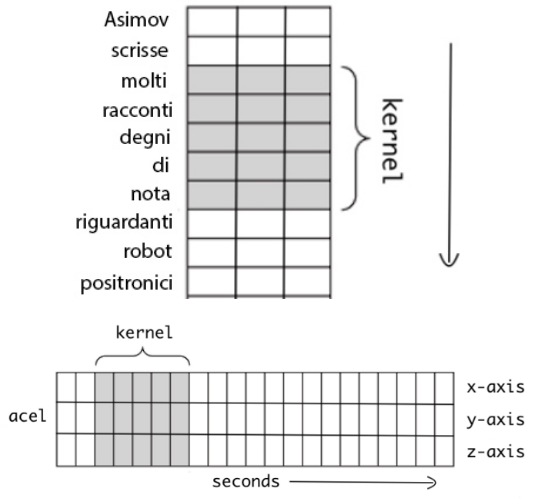
\includegraphics[width=\linewidth]{images/1D_convolution.png}
    \caption{Example of the 1D convolution.}
    \label{fig:1D_convolution}
    \vspace{-10pt}
\end{wrapfigure}
In fact, if we consider text, we can represent each word as a vector of fixed lenght (using word embeddings) and stack these vectors to form a 2D matrix, where each row corresponds to a word in the sequence. Then we can apply 1D convolutions along the temporal dimension (the rows) to capture the relationships between words in the sequence.

The discete 1D convolution is defined as:
\begin{equation}
    (x * w)(n) = \sum_{i=0}^{k-1} x(n-i) w(i)
\end{equation}
Where \textbf{x} is our input vector of lenght \textbf{n}, and \textbf{w} our kernel of lenght \textbf{k}.

\begin{infobox}[Note]
    In the convolution formula we have $x(n - i)$, which implies that the kernel accesses only past values of the input signal. This corresponds to a \textit{causal convolution}, meaning that the output at time $n$ depends only on the current and previous inputs. This property is crucial for sequence modeling tasks, where future information should not be used to predict the next element in the sequence.
\end{infobox}
    
\subsection{Dilated Convolution}
A major disadvantage of using CNNs for sequence modeling is that, in order to achieve a long effective history size (the \textbf{receptive field}), we need an extremely deep network or very large filters. This increases the number of parameters, leading to more complex training, and the network depth can also cause problems such as vanishing or exploding gradients.

\begin{wrapfigure}{r}{0.3\textwidth}
    \centering
    \vspace{-10pt}
    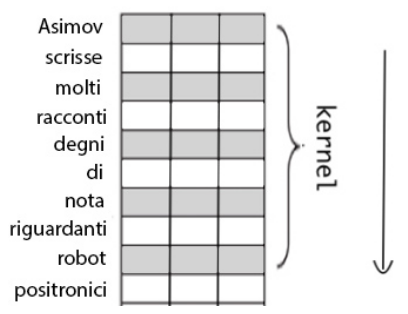
\includegraphics[width=\linewidth]{images/dilatation.png}
    \caption{Example of Dilated Convolution.}
    \label{fig:dilatation}
    \vspace{-10pt}
\end{wrapfigure}

To mitigate this problem we can increase the receptive field using \textbf{dilated convolution}, which introduces gaps between kernel elements to cover a wider input region without increasing the number of parameters.
\begin{equation}
    (x * w)(n) = \sum_{i=0}^{k-1} x(n-d*i) w(i)
\end{equation}
where $d$ is the \textbf{dilation factor}

\newpage
\subsection{Casual Convolution}
\begin{wrapfigure}{r}{0.3\textwidth}
    \centering
    \vspace{-10pt}
    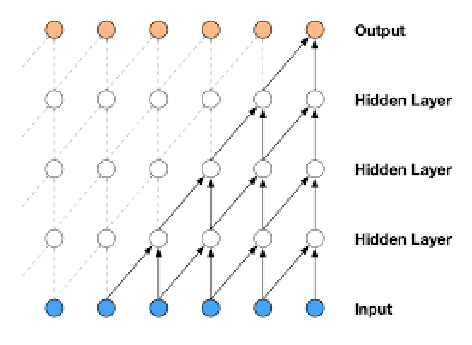
\includegraphics[width=\linewidth]{images/causal_convolution.png}
    \caption{Causal Convolution.}
    \label{fig:causal}
    \vspace{-10pt}
\end{wrapfigure}
A standard convolution can access future input when computing the current output, which may be undesirable for time-series or sequential prediction tasks.

To prevent the model from looking ahead, we can use a \textbf{causal convolution}, which ensures that the output at time step $t$ depends only on inputs from time steps $\leq$ t.

This simple constraint makes CNNs suitable for sequence modeling where causality matters, we will see them again later when discussing autoregressive model.

\subsection{Temporal Convolutional Network}
The \textbf{Temporal Convolutional Network (TCN)} is a model composed of a residual blocks of dilated casual convolution. In TCN each layer use a different \textbf{dilation factor} $d=1,2,4$ and \textbf{filter size} $k=3$
\begin{figure}[H]
    \centering
    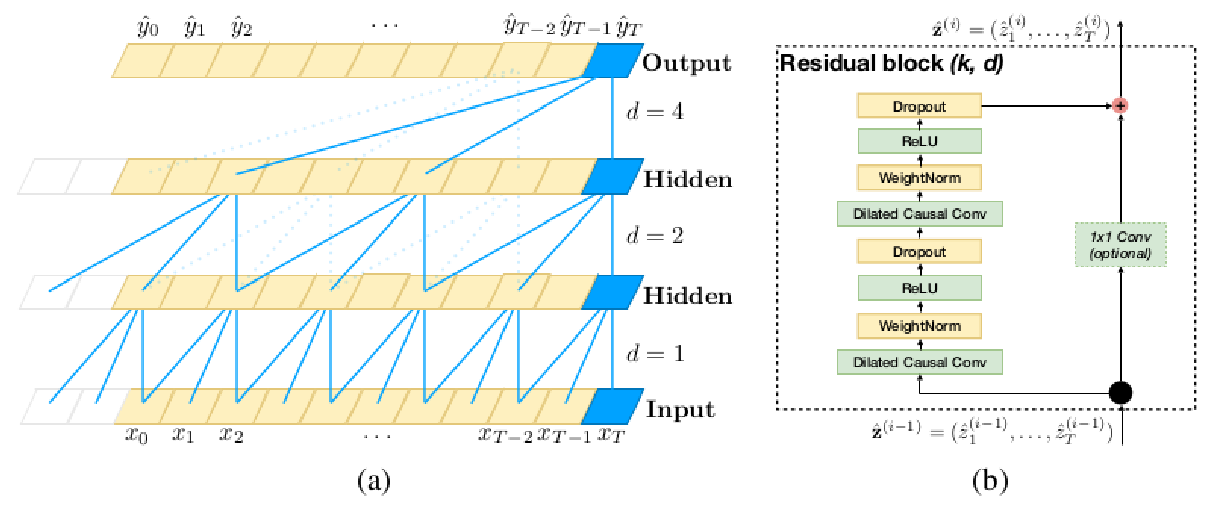
\includegraphics[width=0.9\textwidth]{images/TCN.png}
    \caption{Temporal Convolutional architecture.}
    \label{fig:TCN}
\end{figure}

\begin{infobox}[If the size of the input and output are different?]
    In residual blocks, we need to add the input and the output to form the final output block. To do this, the two elements must have the same size. Therefore, if the input changes its size during the forward pass, we need to apply a convolution to make the input match the size of the output.
\end{infobox}
\begin{infobox}[Effect of the dilated convolution]
    Each element of the output attends to multiple elements of the input, depending on the dilation factor. In this case each element of the outputs attends each element of the input.
\end{infobox}
    
\subsection{TCN vs RNN}
The principal characteristic of TCN compared to RNN are:
\begin{compactitemize}
    \item \textbf{TCN are easier and more stable} to train, they no suffer of vanishing/exploding gradient.
    \item \textbf{Higher effective memory:} longer temporal dependencies can be captured.
    \item \textbf{More parallelizable} and faster on long sequences.
    \item \textbf{Depth=Memory:} receptive field grows with network depth.
    \item Can be equipped by \textbf{explainability modules} 
\end{compactitemize}

\section{Transformer}
Temporal Convolutional Networks (TCNs) are designed to model temporal dependencies in sequential data using a fixed \textit{inductive bias}: local convolutions with an expanding receptive field. This inductive bias is powerful because it enforces causality (outputs depend only on past inputs) and provides stability during training. However, this assumption may not always be appropriate for every problem. In particular, when relevant information is non-local in time or depends on long-range interactions that do not follow a fixed temporal pattern, TCNs may struggle to capture these dependencies. 

For example, in code understanding tasks, the opening of a \texttt{for} loop may influence the value of variables dozens of lines later — a dependency that is difficult to capture using purely local convolutions. This limitation raises the question: can we design a more general architecture that learns how to relate distant elements in a sequence, i.e., how the receptive field should expand, directly from data? The answer is provided by attention-based models, such as Transformers, which can dynamically learn dependencies between distant elements without being constrained by a fixed local receptive field.

\begin{infobox}[What is an inductive bias?]
An \textit{inductive bias} is a set of assumptions that a learning algorithm uses to generalize from training data to unseen data. In the case of TCNs, the inductive bias is that temporal dependencies can be captured using local convolutions with an expanding receptive field. This bias guides the model toward solutions that respect causality and local temporal structure, but it may limit the ability to learn non-local or irregular temporal patterns.
\end{infobox}

\newpage
\subsection{Transformer Architecture}
Transformer network are composed of two main components:
\begin{compactitemize}
    \item \textbf{Encoder}- on the left in the figure.
    \item \textbf{Decoder}- on the right in the figure.
\end{compactitemize}
Each part is built as a stack of $N=6$ layers, forming a deep architecture capable of learning complex dependencies.
\begin{figure}[H]
    \centering
    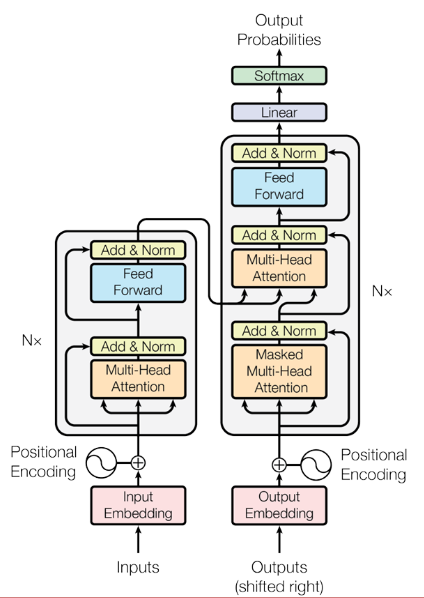
\includegraphics[width=0.5\textwidth]{images/transformer.png}
    \caption{Transformer Architecture.}
    \label{fig:TCN}
\end{figure}
In this course, we will focus on understanding the \textbf{Encoder} part of the Transformer Architecture.

\subsection{Transformer Encoder}
\begin{wrapfigure}{r}{0.2\textwidth}
    \centering
    \vspace{-10pt}
    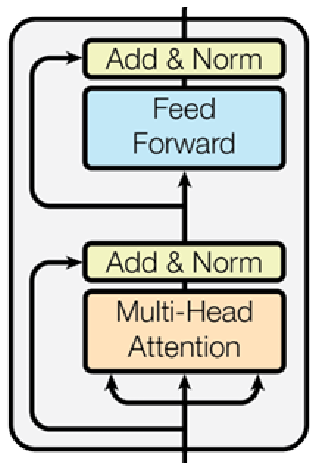
\includegraphics[width=\linewidth]{images/encoder.png}
    \label{fig:encoder}
    \vspace{-10pt}
\end{wrapfigure}
The encoder consists of multiple attention block. The encoder receives an input of embeddings or tokens, each of dimension $d_{model}$, and produces an output of the same shape - with no pooling or dimensionality reduction involved. Usually, we have one token per word or timestep.

Each attention block consist of the following components:
\begin{compactitemize}
    \item A \textbf{Multi-Head Attention (MHA)} layer.
    \item A \textbf{Feed Forward} neural network, composed of two linear layers with a ReLU activation in between.
    \item A \textbf{residual} (or skip) connection after each one of the previus modules, facilitating gradient flow.
    \item \textbf{Layer Normalization} following each residual connection to stabilize training.
\end{compactitemize}

\subsection{Layer Normalization}
Layer Normalization is used to stabilize and speed up training. It normalizes the activations across the features of each example, rather than across the batch as in Batch Normalization. The definition is:
\[
\text{LN}(x) = \frac{x - \mu}{\sigma + \epsilon} \odot \gamma + \beta
\]
where:
\begin{compactitemize}
    \item $\mu=\frac{1}{H}\sum_ix_i$ and $\sigma$ are computed over features.
    \item $\gamma,\beta$ are learnbale affine parameters
    \item normalization is applied \textbf{per token}
\end{compactitemize}
In transformer, LN improves stability in both \textbf{encoder} and \textbf{decoder} stacks.

\begin{infobox}[Difference between LayerNorm and BatchNorm]
    \textbf{Batch Normalization (BatchNorm)} normalizes the activations across the \textit{batch dimension}. For each feature, it computes the mean and variance over the entire mini-batch. This helps to reduce internal covariate shift and can accelerate training, but its behavior depends on the batch size and may be unstable for very small batches.
    
    \textbf{Layer Normalization (LayerNorm)} normalizes the activations across the \textit{feature dimension} for each individual sample. It does not depend on the batch size and is particularly effective in sequence models, such as RNNs and Transformers, where the batch size may vary or be small. LayerNorm ensures consistent normalization for each sample, preserving the temporal or sequential structure.
\end{infobox}

\subsection{The Feed Forward}
The Feed Forward module in Transformers is essentially a classic Multi-Layer Perceptron (MLP). What makes it special is that it is applied \textit{independently to each token} in the sequence. Specifically, for a sequence of token embeddings, the same feed-forward network is applied to each embedding vector without mixing information between different tokens. 

Typically, the feed-forward consists of two linear layers with a non-linear activation function in between (e.g., ReLU). The first layer expands the dimensionality of the token embedding, allowing the network to capture more complex representations, while the second layer projects it back to the original embedding size.

\subsection{The Core Idea of Attention}
In many sequence modeling tasks, not all input elements are equally relevant for producing a given output. Traditional models, such as RNNs or CNNs, process information uniformly, which limits their ability to focus on the most important parts of the input. Attention mechanisms address this limitation by allowing the model to dynamically assign weights to different input elements according to their relevance in the current context. Intuitively, at each step the model asks: ``Which tokens should I pay more attention to right now?''

Formally, for a sequence of input vectors \(X = [x_1, x_2, \dots, x_T]\), the attention mechanism produces a new sequence of contextualized representations \(Z = [z_1, z_2, \dots, z_T]\), where each output vector is a weighted combination of all input vectors:
\[
z_t = \sum_i \alpha_{t,i} \, \mathbf{x}_i, \qquad \alpha_{t,i} = \text{softmax}(s_{t,i})
\]
\begin{infobox}[Important]
The attention coefficients \(\alpha_{t,i}\) are not fixed; they are learned functions of the input, computed through dedicated parametric modules. This allows the model to learn dynamically where to focus depending on the specific input sequence.
\end{infobox}

\subsection{Attention as Content-Based Memory Access}

Instead of compressing all context into a single hidden state (RNNs), the model cna directly \textbf{query the entire sequence of inputs}  to retrieve the most relevant information on demand.

It behaves as a form of \textbf{content-based memory access}: retrieval depends on what is stored, not where it is stored.

The main concepts are:
\begin{compactitemize}
    \item The model mantains a set of \textbf{memory slots}, each represented by a \textbf{key-value} pair.
    \item It generates a \textbf{query} vector describing what it is looking for.
    \item Attention computes the \textbf{similarity} between the query and each key.
    \item Retrieved information is a \textbf{weighted combination of the values}.
\end{compactitemize}

\begin{algorithm}[H]
    \caption{Content-based Retrieval}
    \textbf{Require:}query $q$, keys $\{k_i\}$, values $\{v_i\}$
    \For{each memory slot $i$}{
        $s_i \leftarrow \text{similarity}(q, k_i)$\;
    }
    $\alpha \leftarrow \text{softmax}(s)$ \tcp*[r]{attention weights}
    $z \leftarrow \sum_i \alpha_i v_i$ \tcp*[r]{retrieved information}
    \textbf{return} $z$
\end{algorithm}

\begin{wrapfigure}{r}{0.35\textwidth}
    \centering
    \vspace{-10pt}
    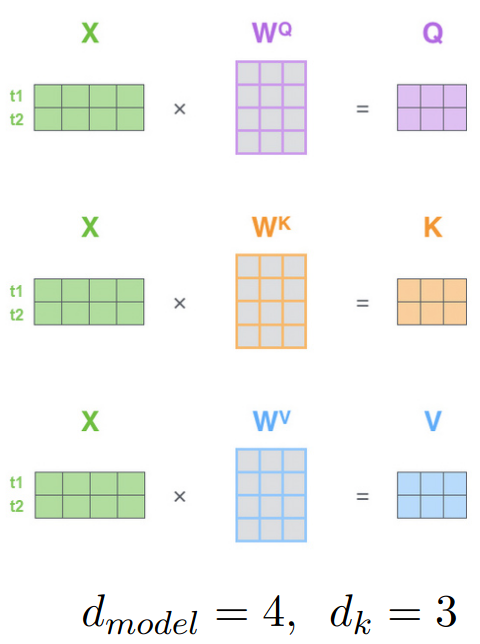
\includegraphics[width=\linewidth]{images/QKV.png}
    \label{fig:QKV}
    \vspace{-10pt}
\end{wrapfigure}

Query, keys, and values are derived from each encoder input vector through linear projections:
\[
Q = X W^Q, \quad K = X W^K, \quad V = X W^V
\]
where \(W^Q, W^K, W^V\) are learnable weight matrices.

These vectors share the dimension \(d_k\), while the input $X$ has dimension \(d_{model}\).

Since all three components originate from the same input ($X$), the attention mechanism is referred to as \textbf{self-attention}.
If the queries, keys, and values come from different sources, it is called \textbf{cross-attention}.

\subsubsection{Single Head Attention}
\begin{wrapfigure}{r}{0.2\textwidth}
    \centering
    \vspace{-10pt}
    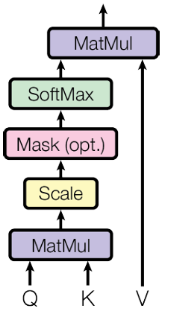
\includegraphics[width=\linewidth]{images/sdpa.png}
    \label{fig:Scaled Dot Product Attention}
    \vspace{-10pt}
\end{wrapfigure}
This mechanism acts as a form of \textbf{content-based memory access}: the model can look back at all inputs and retrieve information on demand.

Formally, the attention operation is defined as:
\[
\text{Attention}(Q, K, V) = \text{softmax}\!\left( \frac{QK^{\top}}{\sqrt{d_k}} \right)V
\]

Here, $Q$, $K$, and $V$ are matrices containing the \textbf{queries}, \textbf{keys}, and \textbf{values}, respectively.  
The dot product $QK^{\top}$ produces a \textbf{similarity matrix} where each entry $(t, i)$ measures how much token $t$ should attend to token $i$.

The dimensionality of $Q$, $K$, and $V$ is $d_k = 64$, which serves as a \textbf{scaling factor} to prevent the dot product from growing too large in magnitude—avoiding saturation of the softmax function that would lead to very small gradients.

\begin{infobox}[Note]
    The softmax is applied row-wise, so that each row of the similarity matrix sums to 1. This ensures that the attention weights for each query form a valid probability distribution over the keys.
\end{infobox}

\subsubsection{Multi-Head Attention}
\begin{wrapfigure}{r}{0.25\textwidth}
    \centering
    \vspace{-10pt}
    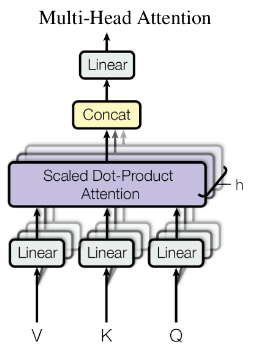
\includegraphics[width=\linewidth]{images/mha.png}
    \label{fig:MHA}
    \vspace{-10pt}
\end{wrapfigure}
The linear projections and the attentions are repeated in parallel multiple times (e.g, h=8), each using a distinct set of weights.

The resulting outputs, each of dimension $d_k$, are then concatenated and passed through a linear layer, which projects the final result to match the dimensionality of $d_{model}$.
Formally, Multi-Head Attention is defined as:
\[
\text{MHA}(Q, K, V) = \text{Concat}(\text{Z}_1, \dots, \text{Z}_h) W^O
\]
where each $Z$ is computed as:
\[
\text{Z}_i = \text{Attention}(X W_i^Q, X W_i^K, X W_i^V)
\]

\begin{figure}[H]
    \centering
    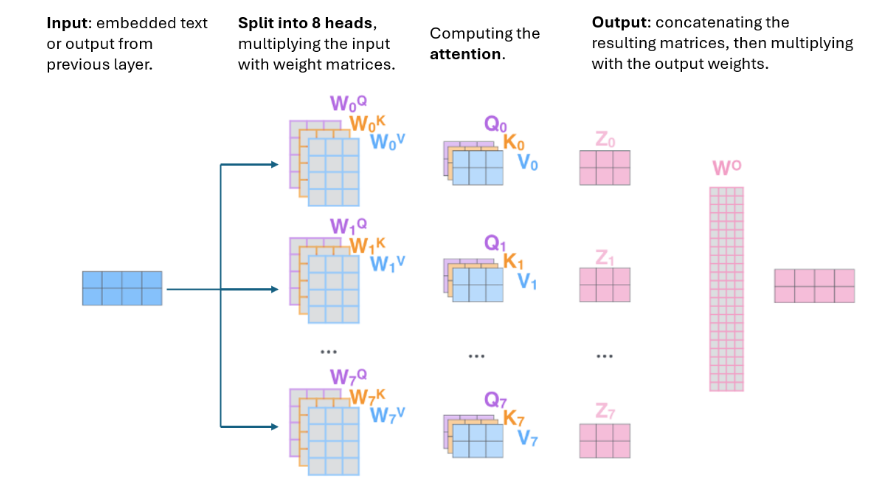
\includegraphics[width=0.9\textwidth]{images/mha2.png}
    \caption{Multi Head Attention.}
    \label{fig:MHA2}
\end{figure}

\begin{infobox}[The problem of concatenate]
    When we use a Multi-Head Attention with $h$ heads, each head produces an output of dimension $d_k$. When we concatenate these outputs, the resulting vector has a dimension of $h \times d_k$. To ensure that the final output of the Multi-Head Attention matches the original input dimension $d_{model}$, we apply a linear transformation using a weight matrix $W^O$ of size $(h \times d_k) \times d_{model}$. This projection step is crucial for maintaining consistency in dimensionality throughout the Transformer architecture.
\end{infobox}

\subsection{From Token Representation to classification}
The encoder outputs a sequence of contextualized token representations, each representing a contextualized version of the corresponding input token. To perform \textbf{classification}, this sequence must be reduced to a single representation. There are two common strategies:
\begin{compactitemize}
    \item \textbf{Average Pooling:} Take the mean of all token embeddings
    \[
    z_{\text{avg}} = \frac{1}{T} \sum_{t=1}^{T} \mathbf{z}_t
    \]
    and feed it to a MLP classifier.
    \item \textbf{[CLS] Token:} Introduce a special classification token prepended to the input sequence. Its final embedding $z_{[CLS]}$ is used as the global representation and passed therough an MLP for classification.
\end{compactitemize}

\subsection{Summary: From TCN to Transformers}

Both TCNs and Transformers are powerful architectures for modeling sequential data, but they rely on different inductive biases and mechanisms.

\begin{compactitemize}
    \item \textbf{Temporal Convolutional Networks (TCN):}
    \begin{compactitemize}
        \item Model temporal dependencies via \textbf{causal and dilated convolutions}.
        \item Capture \textbf{local-to-mid-range temporal structure} efficiently.
        \item \textbf{Stable and easy to train}.
    \end{compactitemize}
    
    \item \textbf{Transformers:}
    \begin{compactitemize}
        \item Model dependencies through \textbf{attention}.
        \item No fixed receptive field — can learn \textbf{arbitrary long-range relations}.
        \item Naturally handle \textbf{multimodal and non-sequential contexts}.
        \item Foundation of modern architectures (\textbf{BERT, GPT, ViT, etc.}).
    \end{compactitemize}
\end{compactitemize}

\textbf{Takeaway:} TCNs impose a \textbf{structured inductive bias}; Transformers learn to \textbf{discover structure directly from data}.

\section{Loss Functions for Regression}
When training models for regression tasks, the choice of loss function is crucial as it directly influences the model's learning process and performance. Here are some commonly used loss functions for regression:
\begin{compactitemize}
    \item The \textbf{Mean Squared Error (MSE)} loss is defined as:
    \[
    \   text{MSE} = \frac{1}{N} \sum_{i=1}^{N} (y_i - \hat{y}_i)^2
    \]
    This loss penalizes large errors more strongly due to the squaring of the differences, making it sensitive to outliers. It is also smooth and differentiable, which is beneficial for optimization.
    \item The \textbf{Mean Absolute Error (MAE)} loss is defined as:
    \[
    \text{MAE} = \frac{1}{N} \sum_{i=1}^{N} |y_i - \hat{y}_i|
    \]
    This loss treats all errors equally, making it more robust to outliers compared to MSE. However, it is less sensitive to small errors and can be less smooth, which may affect optimization.
\end{compactitemize}

\subsection{From Regression to Classification via Binning}
In most cases, predicting continuous values directly can be challenging. An alternative approach is instead of predicting continuos values directly (regression), we can discretize the target into intervals (called \textbf{bins}) and train a model to classify which interval the target belong to.

Let's see an example of age prediction from an image:
\begin{compactitemize}
    \item \textbf{Target variable:} age $\in [0, 100]$
    \item \textbf{Discretization:} Define $K$ bins, e.g.:
    \[
    [0-10], [10-20], [20-30], \dots, [90-100]
    \]
    \item \textbf{Training:} Train a classifier with $K$ output classes (one per age interval).
    \item \textbf{Prediction:} The final age prediction can be:
    \begin{compactitemize}
        \item The \textbf{center of the predicted bin}, e.g., $25$ for $[20-30]$, or
        \item A \textbf{weighted average of bin centers} using class probabilities.
    \end{compactitemize}
\end{compactitemize}

Let's see why converting a regression task into a classification problem can be useful:
\begin{compactitemize}
    \item By discretizing the target variable into bins, we can train a \textbf{classifier} using standard \textbf{cross-entropy loss}.
    \item This approach naturally allows us to \textbf{capture uncertainty} through the predicted probability distribution across bins, giving more informative predictions than a single point estimate.
\end{compactitemize}

\subsection{Limitations of MSE and MAE}
Both MAE and MSE assume \textbf{symmetric errors}: overestimating and underestimating the target by the same amount incur equal penalties. However, in many real-world applications, the cost of overestimation and underestimation may differ significantly. For example:
\begin{compactitemize}
    \item In financial forecasting, overestimating revenue may lead to overspending, while underestimating may result in missed opportunities.
    \item In medical diagnosis, overestimating the severity of a condition may lead to unnecessary treatments, while underestimating may delay critical care.
\end{compactitemize}
We may want to estimate not a single "average" value, but a range of possible outcomes, this motivates the use of \textbf{Quantile Loss}.

\subsection{Understanding Quantiles}
\begin{wrapfigure}{r}{0.35\textwidth}
    \centering
    \vspace{-10pt}
    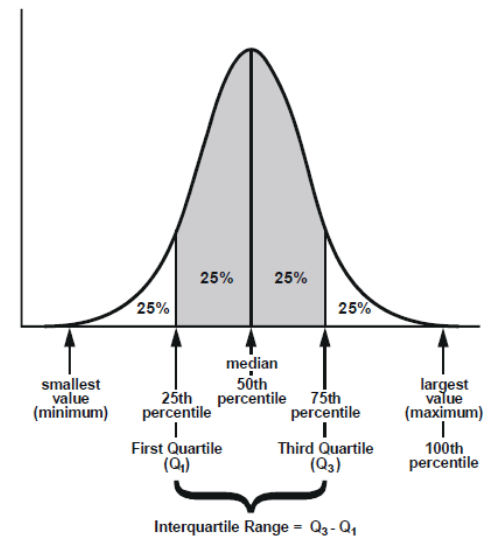
\includegraphics[width=\linewidth]{images/dis.png}
    \label{fig:MHA}
    \vspace{-10pt}
\end{wrapfigure}
The $\tau$-quantile of a distribution is the value $q_{\tau}$ such that $P(Y \le q_{\tau}) = \tau$.
Let's see some examples:
\begin{compactitemize}
    \item The $0.5$-quantile (median) is the value that splits the distribution in half: $50\%$ of values are below it, and $50\%$ are above it.
    \item The $0.25$-quantile (first quartile) is the value below which $25\%$ of the data fall.
    \item The $0.75$-quantile (third quartile) is the value below which $75\%$ of the data fall.
    \item The $0.1$-quantile is the value below which $10\%$ of the data fall.
\end{compactitemize}

\begin{infobox}[Note]
    In gaussian distribution, mena, median and mode are all the same value, but in general this is not true.
\end{infobox}

\subsection{Quantile Loss Function}
The goal of quantile regression is to estimate the $\tau$-quantile of the target variable given the input features. The quantile loss function, is defined as:
\[
L_{\tau}(y, \hat{y}) = \begin{cases}
\tau (y - \hat{y}) & \text{if } y > \hat{y} \\
(1 - \tau) (\hat{y} - y) & \text{if } y \leq \hat{y}
\end{cases}
\]
where: 
\begin{compactitemize}
    \item $y$ is the true target value and the $\hat{y}$ is the etimate
    \item $\tau \in (0, 1)$ is a \textbf{hyperparameter} that controls which quantile we want to estimate.
\end{compactitemize}

Let's see some questions:
\begin{compactitemize}
    \item What happens when $\tau = 0.5$?  
    The Quantile Loss collapses to the \textbf{Mean Absolute Error (MAE)}.
    
    \item How are errors weighted when $\tau = 0.9$?  
    Underestimations ($\hat{y} < y$) are penalized $9\times$ more than overestimations, so it’s more convenient for the model to slightly overpredict.
    
    \item When $\tau = 0.9$, is the model encouraged to underestimate or overestimate the target?  
    It tends to \textbf{overestimate}, aligning predictions with the 90th percentile.
\end{compactitemize}

In summary, the main properties of Quantile Loss are:
\begin{compactitemize}
    \item \textbf{Asymmetric}: underestimations and overestimations are penalized differently.
    \item Encourages the model to predict the \textbf{$\tau$-quantile} of the $Y$.
\end{compactitemize}
The intuition is that the model "pays" more for errors on one side of the prediction, depending on the chosen quantile $\tau$.